\chapter{Implementácia}

Po preskúmaní triangulačných algoritmov sme sa v našej práci rozhodli venovať čo najkvaitnejšiemu
prevedeniu triangulácie s menším dôrazom na rýchlosť výpočtu. Ako základnú štruktúru sme použili 
postup, ktorí uviedli autori článku \cite{hilton1996marching}. Tento algoritmus využíva 
\textit{Delaunayovu podmienku} predstavenú v kapitole \ref{kap:delaunay_triangulation}.
Daný algoritmus je implementovaný ako prechod cez frontu, v ktorej sa na úvod nachádzajú
hrany počiatočného trojuholníka, v každom kroku vyberieme z fronty jednu hranu $E$ a pre túto
hranu vykonáme nasledujúcu postupnosť krokov:
\begin{enumerate}
    \item{Vytvoríme vrchol $x_{proj}$ tak, ako sme opísali v kapitole \ref{kap:marching_triangles}, teda 
    ako bod ležiaci v kolmej vzdialenosti $k$ od stredu hrany $E = (x_i, x_j)$ v rovine susedného 
    trojuholníka $T$.}
    \item{Nájdeme vrchol $x_{new}$ ako vrchol, ktorý leží na povrchu a je najbližší k bodu $x_{proj}$. 
    Platí teda, že $F(x_{new}) = 0$.}
    \item{Skončíme ak je splnená jedna z nasledujúcich možností:
    \begin{itemize}
        \item{Vrchol $x_{new}$ leží na hranici, teda medzi hraničnými hranami sa nechádza hrana s vrcholom 
        $x_{new}$.}
        \item{Normála $n_{new}$ trojuholníka $T_{new}$ ktorého vrcholy sú $x_i, x_j, x_{new}$ je opačná ako
        normála $n$ susedného trojuholníka $T$, teda $n_{new} \cdot n < 0$.}
    \end{itemize}
    }
    \item{Pre trojuholník $T_new$ overíme platnosť \textit{Delaunayovej podmienky}, 
    ktorú sme predstavili v kapitole \ref{kap:delaunay_triangulation}, ak podmienka platí
    vykonáme nasledujúce kroky a prejdeme na ďalšiu hranu.
    \begin{itemize}
        \item{Pridáme vrchol $x_{new}$ medzi hraničné vrcholy.}
        \item{Pridáme trojuholník $T_{new}$ do meshu.}
        \item{Pridáme hrany $(x_i, x_{new})$ a $(x_j, x_{new})$ do fronty s hranami.}
    \end{itemize}
    }
    \item{
        Ak podmienka neplatí overíme platnosť \textit{Delaunayovej podmienky} pre Trojuholníky 
        $T_{prev}$, ktorého vrcholy sú $x_i, x_j, x_{prev}$ a $T_{next}$, ktorého vrcholy sú 
        $x_i, x_j, x_{next}$, kde $x_{prev}$ a $x_{next}$ sú hraničné vrcholy, $x_{prev}$ 
        je sused vrchola $x_i$, $x_{next}$ je sused vrchola $x_j$. Ak niektorý z nich podmienku
        spĺňa, vykonáme preň body zo kroku 4 a prejdeme na ďalšiu hranu.
    }
    \item{
        Ak všetky trojuholníky $T_{new}$, $T_{prev}$ ani $T_{next}$ nespĺňajú podmienku, potom 
        ak \textit{Delaunayova guľa} obsajuhe hraničný vrchol $x_{overlap}$ nejakého hraničného 
        trojuholníka $T_{overlap}$, ktorý je rovnako orientovaný ako hraničný trojuholník T, teda
        platí $n*n_{overlap} > 0$, potom overíme platnosť \textit{Delaunayovej podmienky} pre 
        trojuholník $T_{overlap}$ kde $x_{overlap}$ je najbližší k hrane E zo všetkých hraničných
        vrcholov, ktoré sa nachádzajú v Delaunayovej guli. Ak podmienku spĺňa aplikujeme naň body z 
        kroku 4 a prejdeme na ďalšiu hranu.
    }
    \item{
        Ak žiadny trojuholník nebol pridaný do meshu, testovanie hrany E skončíme.
    }
\end{enumerate}

Tento algoritmus používame v našej práci ako základnú štruktúru a pridávame do neho ďalšie podmienky 
a postupy na skvalitnenie výslednej triangulácie. V neadaptívnej verzií volíme vzdialenosť $k$ ako 
výšku rovnostranného trojuholníka so stranou dĺžky zadanej ako vstupný parameter algoritmu, teda 
$\frac{\sqrt{3}}{2}*strana$.

\section{Problémy základnej formy algoritmu}

V tejto kapitole popíšeme aké problémy vnímame v základnej forme algoritmu a navrhneme riešenia, v 
ďalšej kapitole popíšeme implementáciu našich riešení.

Ako prvý problém vnímame nespájanie bodov, ktoré sa k sebe nachádzajú blízko. Ako dôsledok vznikajú neskôr
úzke alebo malé trojuholníky. Príklad takétoho správania môžeme vidieť na obrázku \ref{obr:first_problem}.
Keďže trojuholník $T_{new}$ spĺňa Delaunayovu podmienku, tak podľa základného algoritmu pridáme trojuholník
do meshu, avšak zdalo by sa nám správne aby sme vytvorili a pridali do meshu trojuholník 
$x_i, x_j, x_{prev}$. 

Našim nevrhovaným riešením je zväčšiť polomer \textit{Delaunayovej gule} na $1.1-$násobok pôvodného polomeru,
zároveň pridávame v okolí vrchola $x_{new}$ guľu s polomerom $0.3-$násobku dĺžky strany trojuholníka a overujeme 
body vnútri oboch týchto gulí. Ak sa v ňom vyskytne nejaký bod, pokúsime sa vytvoriť trojuholník s týmto bodom.
Tento postup ilustrujeme na obrázku \ref{obr:first_problem_solution}.

\begin{figure}
    \centerline{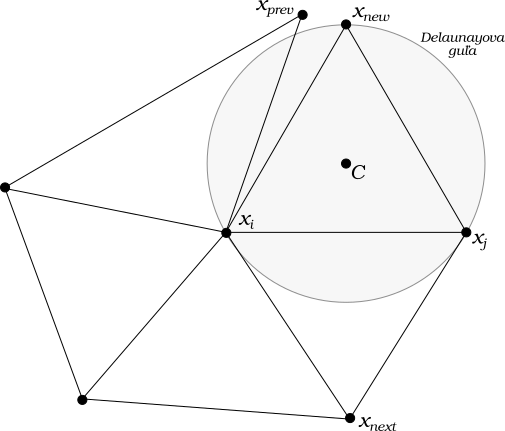
\includegraphics[width=0.5\textwidth]{images/first_problem}}
    \caption[Trojuholník $T_{new}$ spĺňa Delaunayovu podmienku]{Trojuholník $T_{new}$ spĺňa Delaunayovu podmienku}
    %id obrazku, pomocou ktoreho sa budeme na obrazok odvolavat
    \label{obr:first_problem}
\end{figure}

\begin{figure}
    \centerline{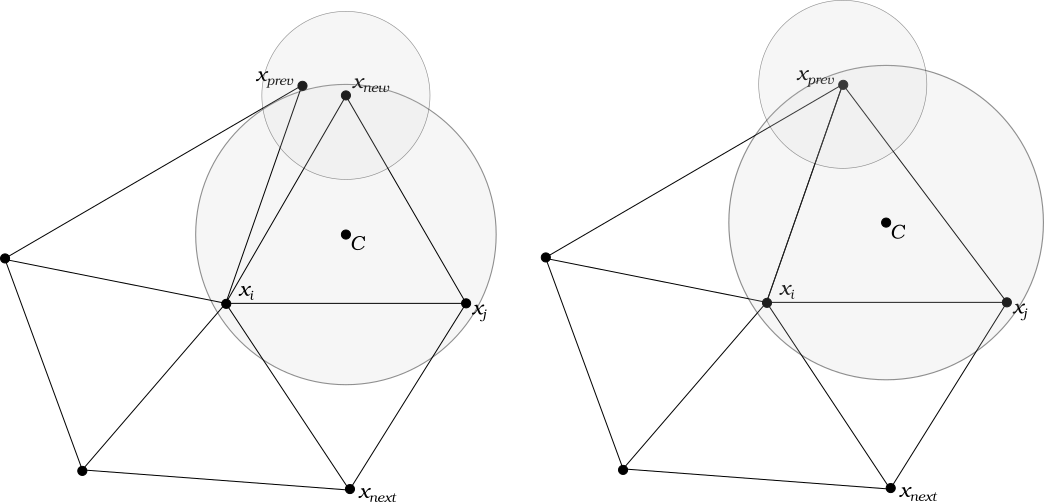
\includegraphics[width=1\textwidth]{images/first_problem_solution}}
    \caption[Trojuholník $T_{new}$ nespĺňa upravenú Delaunayovu podmienku]{Trojuholník $T_{new}$ nespĺňa upravenú Delaunayovu podmienku}
    %id obrazku, pomocou ktoreho sa budeme na obrazok odvolavat
    \label{obr:first_problem_solution}
\end{figure}



